
\documentclass[a4paper,12pt]{article}

\usepackage{ucs}
\usepackage[utf8x]{inputenc}
%\usepackage[latin1]{inputenc}
\usepackage[T1]{fontenc}

\usepackage[french]{babel}

\pagestyle{plain}

\usepackage{graphicx}
\usepackage{subfigure}
\DeclareGraphicsExtensions{.pdf,.eps,.jpg,.png,.gif}

\usepackage{color}
\definecolor{grey}{rgb}{0.9,0.9,0.9}
\definecolor{teal}{rgb}{0.0,0.5,0.5}
\definecolor{violet}{rgb}{0.5,0,0.5}

\usepackage{listings}
\usepackage{listingsutf8}
\lstloadlanguages{[Visual]C++}
\lstdefinestyle{listing}{
  language=Java,
  captionpos=t,
  inputencoding=utf8/latin1,
  extendedchars=true,
  resetmargins=true,
  xleftmargin=-60pt,
  xrightmargin=-70pt,
%  frame=single,
  numbers=left,
  numberstyle=\tiny,
  numbersep=5pt,
  breaklines=true,
  breakatwhitespace=true,
  showspaces=false,
  showstringspaces=false,
  showtabs=false,
  tabsize=2,
  basicstyle=\footnotesize\ttfamily,
  backgroundcolor=\color{grey},
  keywordstyle=\color{blue}\bfseries,
  commentstyle=\color{teal},
  identifierstyle=\color{black},
  stringstyle=\color{red},
  numberstyle=\color{violet},
}
\lstset{style=listing}

%%%%%%%%%%%%%%%%%%%%%%%%%%%%%%%%%%%%%%%%%%%%%%%%%%%%%%%%%%%%

\author{
  Quentin \textsc{Augrain}, Florent \textsc{Mallard} \\ \\
  INSA de Rennes \\
  5INFO
}

\title{Projet de Modélisation et Ingénierie du vivant}

\begin{document}
\maketitle

\section{Tutoriel}

Question 1: Comme indiqué dans les commentaires de la fonction, il y a deux fonctions dnas la boucle :
\begin{itemize}
    \item Bouger le monde;
    \item Afficher le monde.
\end{itemize}

Cela signifie que la fonciton va tout d'abord calculer le prochain mouvement, pour ensuite afficher la nouvelle position. Pour le moment, la phase de calcul n'est pas implémentée et rien ne bouge dans la simulation.

Question 2: Rien ne se passe. En effet même si nous calculons maintenant les forces, nous ne les appliquons pas au mesh, ce qui résulte en un écran fixe.
\begin{figure}
  \centering
  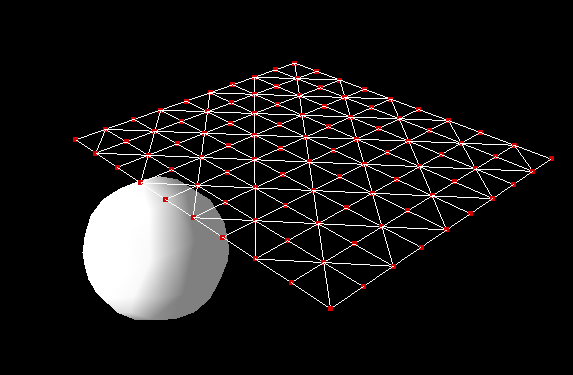
\includegraphics{q2.png}
  \caption{Aucun changement n'est visible même si les forces changent.}
  \label{fig:q2}
\end{figure}

Question 3: Maintenant que nous appliquons les forces, le mesh tombe et finit par disparaitre de l'écran.

Question 4 : Afin de fixer le premier rang de particules, il nous faut nullifier les forces de ces partiules. Nous avons compté 10 particules sur ce rang, nous avons donc ajouté une boucle comme montré sur la \textsc{Figure} \ref{fig:q4}.
\begin{figure}
  \centering
  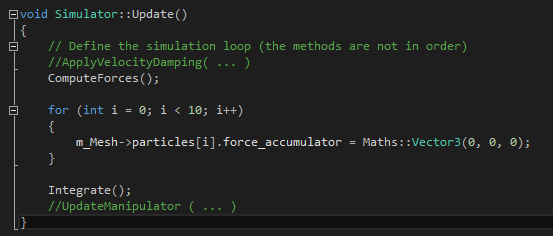
\includegraphics{q4.png}
  \caption{Le premier rang reste fixe.}
  \label{fig:q4}
\end{figure}

Question 5 : Le comportement est pour le moins étrange, car les particules oscillent de plus en plus jusqu'à disparaître.
La \textsc{Figure} \ref{fig:q5} montre notre implémentation.
\begin{figure}
  \centering
  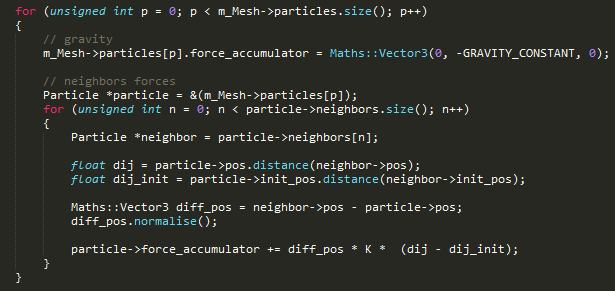
\includegraphics{q5.png}
  \caption{Mise à jour des voisins pour chaque particule.}
  \label{fig:q5}
\end{figure}

Question 6 : Le paramètre dt définit la vitesse de la simulation à travers le nombre d'itérations à  chaque fois. Une valeur plus petite correspond donc à une simulation plus rapide, car on calcule la position et les forces après un instant plus grand, le mouvmenent a donc été plus important.
K définit la rigidité. Celle-ci va aider à obtenir l'effet de rideau désiré. Sachant cela, nous n'avons pas réussi à stabiliser la simulation.

Question 7 : Le CPU est bien plus actif après que nous ayons implémenté la boucle, car même si nous n'affichons pas les résultats les calculs se font.

Question 8 : En amortissant la chute des particules, nous arrivons à stabiliser la simulation. L'amortissement simule l'interaction des particules avec l'air ambiant.%TODO Image(s) de la chute et/ou du résultat
%\begin{figure}
%  \centering
%  \includegraphics{}
%  \caption{Le mesh ressemble à un rideau pendant.}
%  \label{fig:}
%\end{figure}

Question 9 : 	Avec dt = 1/200, K = 300, et n = 20, nous arrivons à une simulation stable.

Question 10 : Le modèle de Mass-Spring-Damper est assez simple à utiliser dès lors que les formules à appliquer sont à disposition. En revanche, pour obtenir une simulation stable, le moindre écart dans les paramètres peut créer une simulation tout à fait exotique.

\section{TP2}

Question 1 : Baisser la valeur d'amortissement résulte en une accélération de la chute et en une baisse de la stabilité. La vitesse relative est simplement une soustraction de vecteurs.

Question 2 : Afin de simuler le sol, nous implémentons une limite de hauteur en dessous de laquelle les particules ne peuvent descendre, ayant pour effet de simuler un plan. %TODO image sol + code
%\begin{figure}
%  \centering
%  \includegraphics{}
%  \caption{Implémentation du sol.}
%  \label{fig:}
%\end{figure}

%\begin{figure}
%  \centering
%  \includegraphics{}
%  \caption{Rideau tombé sur le sol.}
%  \label{fig:}
%\end{figure}

Question 3 : Nous avons simplement changé la couleur de notre manipulator, que nous montrons ci-dessous : %TODO
%\begin{figure}
%  \centering
%  \includegraphics{}
%  \caption{Le manipulateur est maintenant de couleur rouge.}
%  \label{fig:}
%\end{figure}


Question 4 : Le coefficient C, s'il est négatif, créé une attraction entre le manipulator et le mesh. En revanche, s'il est positif, les deux objets se repoussent.

Question 5 : %TODO code
%\begin{figure}
%  \centering
%  \includegraphics{}
%  \caption{Ajout du client haptique.}
%  \label{fig:}
%\end{figure}

Question 6 :%TODO code
%\begin{figure}
%  \centering
%  \includegraphics{}
%  \caption{Ajout de la force en retour.}
%  \label{fig:}
%\end{figure}

Question 7 :%TODO code
%\begin{figure}
%  \centering
%  \includegraphics{}
%  \caption{Ajout du clic avec le client haptique.}
%  \label{fig:}
%\end{figure}

Question 8 :%TODO code
%\begin{figure}
%  \centering
%  \includegraphics{}
%  \caption{Le mesh resemble à un rideau pendant.}
%  \label{fig:}
%\end{figure}

Question 9 :%TODO scrshot
%\begin{figure}
%  \centering
%  \includegraphics{}
%  \caption{Mesh représentant un foie.}
%  \label{fig:}
%\end{figure}

Question 10 :%TODO scrshots
%\begin{figure}
%  \centering
%  \includegraphics{}
%  \caption{Le mesh resemble à un rideau pendant.}
%  \label{fig:}
%\end{figure}

Question 11 :

\end{document}
